\section{Abstract Data Model}\label{motivation}

%\subsection{Introduction}\label{introduction}

The previous sections of this chapter established the motivation for building computational pipelines for spatio-temporal analysis of team sport and modelled the game of \afl{} as well as the player feedback systems involved. This section will model the types of sensor data available that could power such an approach.

Traditionally, only summary statistics such as total number of goals were recorded. However, the
advent of sport databases has allowed a much richer set of data to be
collected, such as the time and players involved in every pass.
Recently, the National Basketball Association (NBA) have installed
computer vision technology that tracks the precise location of the ball
and every player on the court. Similarly, AFL players are also tracked, albeit through a different technological means. In AFL, players wear tracking devices during the game that have a
GPS chip for tracking position, in addition to sensors for measuring
acceleration, orientation, and (optionally) heart rate.

It is not just coaches that are interested in these data. Sport fans,
betting markets, sport reporters, and sport researchers are also
stakeholders with an interest in the data collected. Each stakeholder
requires access to different kinds of data depending on the objective
they wish to achieve, and their intended method of analysis.

Clearly, the detailed player tracking data available today provides much
more detail than the simple counts that have been recorded historically.
However, what lacks is a consistent language for expressing the detail
and type of data each stake-holder requires, and which types of analysis
the data can support.

Further complicating the issue is that of measurement errors inherent to
the sport data collection technology used. For sound sport research,
it is vital that sources of errors are known so that errors can be dealt
with in a rigorous manner using appropriate statistical and inference
techniques rather than simply neglected \cite{Hughes2004}.

% Not a meta-model!
% \begin{figure}[htbp]
% \centering
% 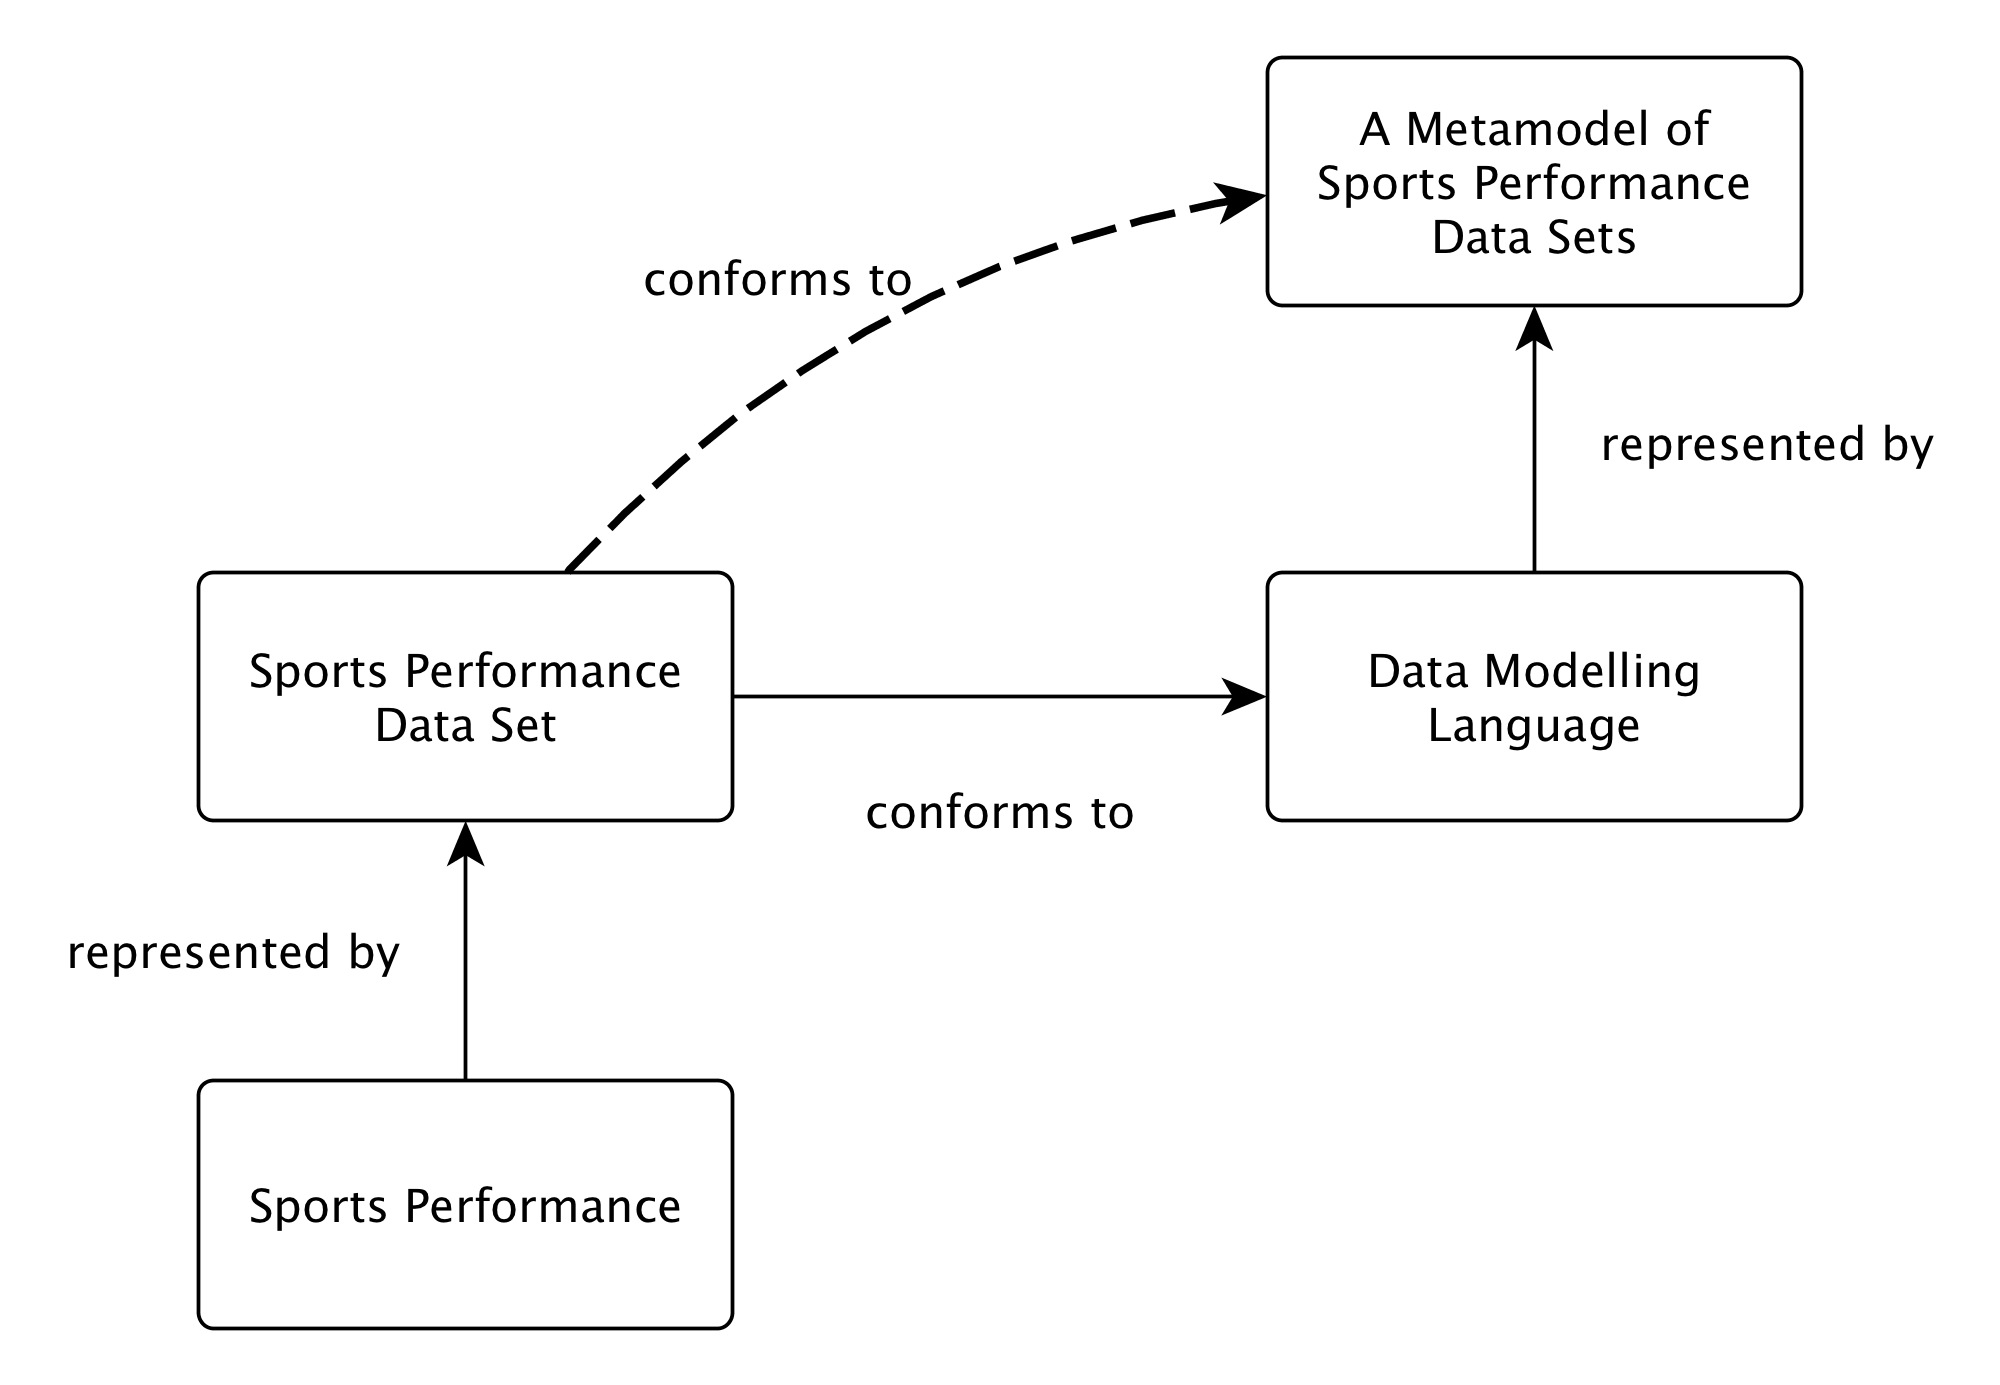
\includegraphics[width=\linewidth]{sports_metamodel}
% \caption[Metamodelling relationship (shown as dashed line)
% \label{fig:sports_metamodel}]{Metamodelling relationship (shown as
% dashed line)\footnotemark{} \label{fig:sports_metamodel}}
% \end{figure}
% \footnotetext{This figure is drawn in the same style as the meta-model
%   diagram in G. G\'enova, ``What is a metamodel: the OMG's metamodeling
%   infrastructure,'' 2009.
%   \url{http://www.ie.inf.uc3m.es/ggenova/warsaw/part3.pdf}}

% We present our model as a ``metamodel'', as it describes the essential
% elements of a language that could be used to model sports performance
% datasets. The meta-model relationship is represented as a dashed line
% in \figref{fig:sports_metamodel}.

This section presents an abstract data model that establishes the fundamental data
types involved in sport datasets, with a focus on the ability to describe
spatio-temporal datasets, such as those collected by GPS tracking devices.
This abstract data model is later used to describe concrete data schemas
for specific datasets (\appendixref{appendix:modelling}).

\subsection{Related Work}\label{related-work}

In 1946, Stevens proposed classifying measurements as Nominal, Ordinal,
Interval, and Ratio scales \cite{stevens1946scales}. The scale
classification was defined with respect to two competing concerns: transformations
that could be applied to the scale whilst still preserving its essential
relationships (for example, player identification numbers are on a
nominal scale, and can be arbitrarily re-assigned); and statistical
operations that could be meaningfully be performed upon the scale
(interval and ratio scales such as player speed allow taking the
mean, but it is meaningless to talk about the mean player identification
number).

Stevens' classification model was revolutionary in its realisation that
qualitative measurements and physical measurements could both be
described on the same scale hierarchy, and both permit sound scientific
analysis so long as the limits of the particular scale are respected.
However, Stevens' levels of measurement are not without criticism; in
particular, the limits they place on which statistical operations can
be meaningfully performed, whilst theoretically justified, can be overly
restrictive and unpragmatic in practice \cite{lord1953statistical}.
Stevens' levels of measurement may not be well suited for certain
domains; in 1998, Chrisman identified that Stevens' original levels were
not well suited for cartographic measurements, and proposed additional
levels for Graded membership, Log-interval, Extensive ratio, Cyclic
ratio, Derived ratio, Counts, and Absolute
\cite{chrisman1998rethinking}.

The introduction of low cost positioning sensors that monitor both time
and location has led to the question of how to handle spatio-temporal
data, and the need to distinguish between datasets that merely consist
of separate space and time measurements from those where space and time
are intricately interlinked. Moving object database research \cite{schneider2009moving} attempts to rethink the design of databases to handle the unique challenges posed when storing and querying spatio-temporal data rather than conventional tabular data. Suitably accounting for measurement errors when processing spatio-temporal data requires
careful selection of techniques based upon the type of data queries
performed \cite{cao2006spatiotemporal}.

In practice, most spatio-temporal data models either: provide full
support for the spatial aspect of the data, with secondary consideration
given to the temporal aspect (for example, Geographic Information
Systems); or focus on the temporal aspect of the data, with secondary
consideration of the spatial dimensions (for example, time series
analysis). These differences are so fundamental, that in the design of
the \textit{R} software package ``Spacetime'', multiple representations are
provided to deal with the different forms of spatio-temporal data
\cite{pebesma2012spacetime}.

Sport databases are typically designed for a specific sport. This is
surprising, as sport media networks typically cover a range of different sport types,
so one would assume that they could reduce costs by abstracting the
common elements of multiple sport types into a unified structure.
Furthermore, sport researchers require consistent schemas to conduct
meta-analysis. The lack of a common structure has made it difficult for
sport scientists to conduct systematic reviews across multiple sport types,
such as in Cummins et al. \cite{Cummins2013} where inconsistencies of speed
zones, even within the same sport, were noted as a limitation of the
analysis.

% \nb{include recent standardisation work by FIFA? } % done (thanks to VU Player Tracking Workshop 2019).

Despite the growing prominence of sport analytics, very few attempts
have been made to construct a unified model of sport performance data. The Sports Standards Alliance\footnote{\url{http://www.sportsdb.org/sd}}
attempts to promote a standardised schema for sport. However, this
attempt at standardisation is catered to sport fans rather than
coaches or researchers, and hence tends to focus on traditional summary statistics. It includes data fields for in-game events for some types of sport, but support for time dense spatio-temporal data (such as player position tracking data) is limited.


%  don't attempt to model in-game sport
% performance data beyond the traditional summary statistics reported on
% sport matches.

% In his bachelor's thesis, Chang\footnote{L. Chang, ``The Universal
%   Sports Database,'' Bachelor's thesis, Computer Science, Boston
%   College, Massachusetts, 2008.} built a universal sport database using
% common software frameworks and techniques that are well known to
% software engineers.

Motivated by the desire to reduce the burden on clubs to perform custom data processing to integrate with specific tracking providers, FIFA proposed the Electronic Performance and Tracking Systems (EPTS) standard data format\footnote{FIFA, ``EPTS standard data format'' \url{https://football-technology.fifa.com/en/media-tiles/epts-standard-data-format/} Accessed:~2019-02-20}. Notably, the same format is used to support Optical, GPS, or Radio Frequency based tracking data. As the standard is specifically designed for Association Football, it includes meta-data fields for teams, players, sessions, and field dimensions. Rather than enforcing a specific format for the main tracking data, the standard provides fields to specify parsing details such as the field separators so that tracking output format variations are possible while still allowing all variations to be parsed automatically. While providers are free to add additional data fields, unfortunately the standard itself does not make any attempt to standardise reporting of the accuracy of the tracking data (e.g. the Horizontal Dilution of Precision (HDOP) used to report the accuracy of GPS tracking data).

The W3C Semantic Sensor Network Ontology\footnote{W3C, ``Semantic Sensor Network Ontology,'' 2017. \url{https://www.w3.org/TR/vocab-ssn/} Accessed: \dt{2019-05-02}} is the W3C standard for modelling sensor data in an machine-readable format. In the standard, a platform may have multiple sensors, which make observations of (real-world) properties. The standard provides the ability to model the accuracy and precision of sensor readings, and to associate these with operating conditions. Current applications\footnote{W3C, ``On the usage of the SSN ontology,'' 2019. \url{https://w3c.github.io/sdw/ssn-usage/} Accessed: \dt{2019-05-02}} of the standard include Internet of Things, smart cities and environmental sensing.

Gudmundsson and Horton conducted a recent literature review
\cite{Gudmundsson2016} of spatio-temporal sport
analysis techniques, and distinguish between \emph{event logs}
containing data points at the time of just key events (for example the
set of time and location pairs from which goal attempts were made), and
\emph{trajectory} datasets containing regularly sampled data points
(for example player GPS trajectories). In the design of the \textit{R} software
package ``zoo'', \emph{event logs} are classified as \emph{irregular
timeseries}, and \emph{trajectory} data are classified as \emph{regular
timeseries} \cite{Zeileis2005}.

% In theory, the ontology could also be applied to model sport datasets.

As highlighted above, there exists well established theory on measurement
scales, there is research directed towards the challenges of
processing and storing spatio-temporal data, and that there exists
statistical and mathematical work on the proper treatment of errors in
spatio-temporal datasets. The work of Chrisman
\cite{chrisman1998rethinking} demonstrates the necessity of adapting existing
measurement theory to cater to the subtly different properties that
measurement scales acquire when contextualised to a specific domain. The FIFA EPTS standard data format demonstrates the ability to separate the representation of spatio-temporal data from the specific technology used to collect the data; however, does not currently standardise reporting the errors associated with data points. The W3C Semantic Sensor Network Ontology provides a general framework for formally modelling sensors and sensor accuracy, which in theory could be used to model sport sensor data; however, unlike the FIFA EPTS standard data format it has not been designed with the needs of sport specifically in mind. There exist mathematical models for precise treatment of errors in spatio-temporal data, but errors are often neglected by sport practitioners working with real game
data, outside of isolated studies to validate equipment.

%\nb{Todo: Discuss recent work in literature regarding spatio-temporal modelling frameworks and Moving Object Databases. Rationalise why sport deserves its own spatio-temporal model} % Moving object databases briefly discussed. Could include existing modelling frameworks, but too long as is (would be better to talk about sensor )

%\todo{Review W3C Semantic Sensor Networks model and include if relevant \url{https://en.wikipedia.org/wiki/Semantic\_Sensor\_Web\#W3C\_Semantic\_Sensor\_Networks}}

% https://www.w3.org/TR/vocab-ssn/

\subsection{Sensor Model}\label{our-model}

This sub-section provides a means to describe datasets in terms of the sensors that record the data. It bares some high level similarities to the W3C Semantic Sensor Network Ontology (e.g. the need to model platforms consisting of multiple sensors and to describe the accuracy associated with each recorded parameter). However, in contrast to the W3C Semantic Sensor Network Ontology, the focus is on describing the different types of spatio-temporal data encountered in sport (wearable position tracking devices, human data entry, etc.) rather than attempting to provide a machine-readable specification for data interchange of all forms of sensor data.

A sensor measures one or more \emph{sparse} parameters together as a
function of one or more \emph{dense} parameters, for example, a GPS
position sensor collects sparse position measurements as a function of
dense time measurements. To distinguish between interlinked measurements
versus aggregation of different datasets, the model distinguishes between a
\emph{sensor} and a \emph{sensor platform}. A sensor platform is a
collection of heterogeneous sensors. For example, a player monitoring
device may contain both a GPS position sensor, as well as a heart rate
sensor. Modelling these as separate sensors allows modelling the
heart-rate sensor with a different sampling rate to the GPS position
sensor. Note that a \emph{measured parameter} represents a measurement
of some real-world parameter, not the actual real-world parameter
itself. Unlike real-world parameters, measured parameters represent
samples at discrete intervals, and will contain an error due to the
limitation of the sensor used. The proposed model is presented using UML domain
modelling notation in \figref{fig:sensor_platform}.

\begin{figure}[htbp]
\centering
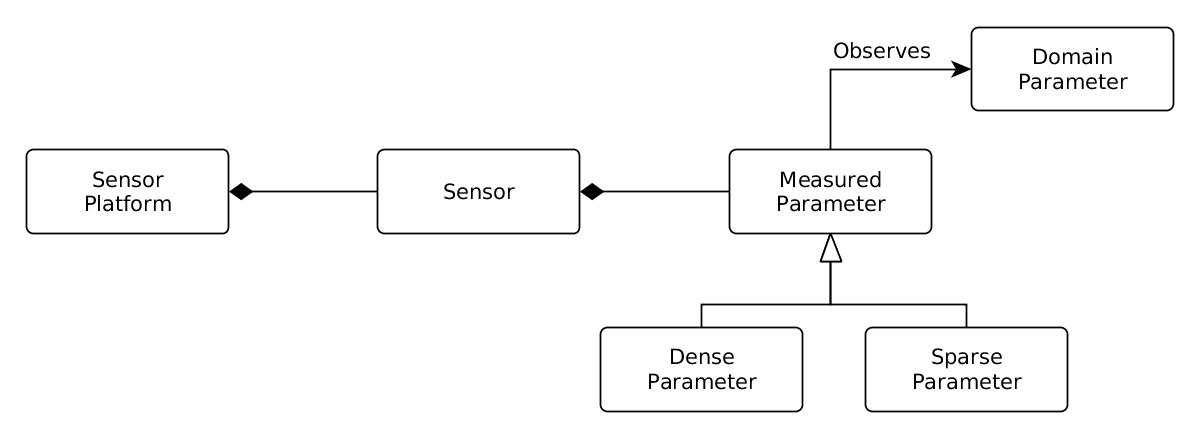
\includegraphics[width=\linewidth]{sensor_platform}
\caption{Abstract Data Model \label{fig:sensor_platform}}
\end{figure}

\begin{figure}[htbp]
\centering
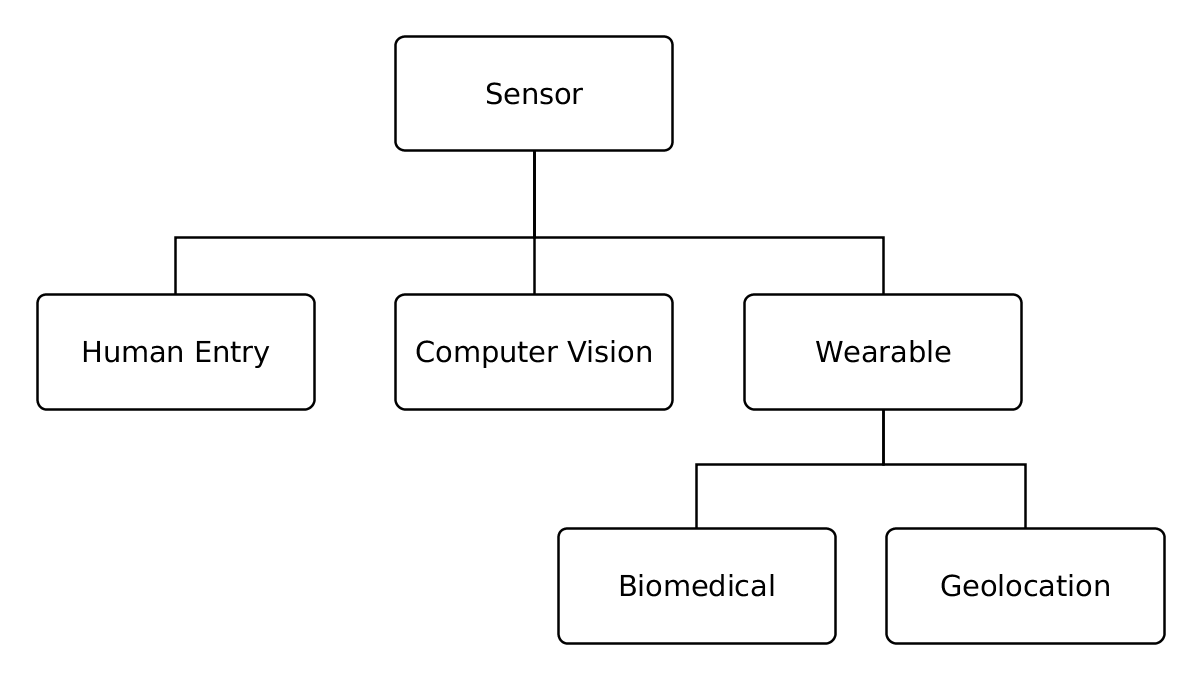
\includegraphics[width=0.8\linewidth]{sensor_platform_sensor_hierarchy}
\caption{Sensor type hierarchy \label{fig:sensor_platform_sensor_hierarchy}}
\end{figure}

\begin{figure}[htb!]
\centering
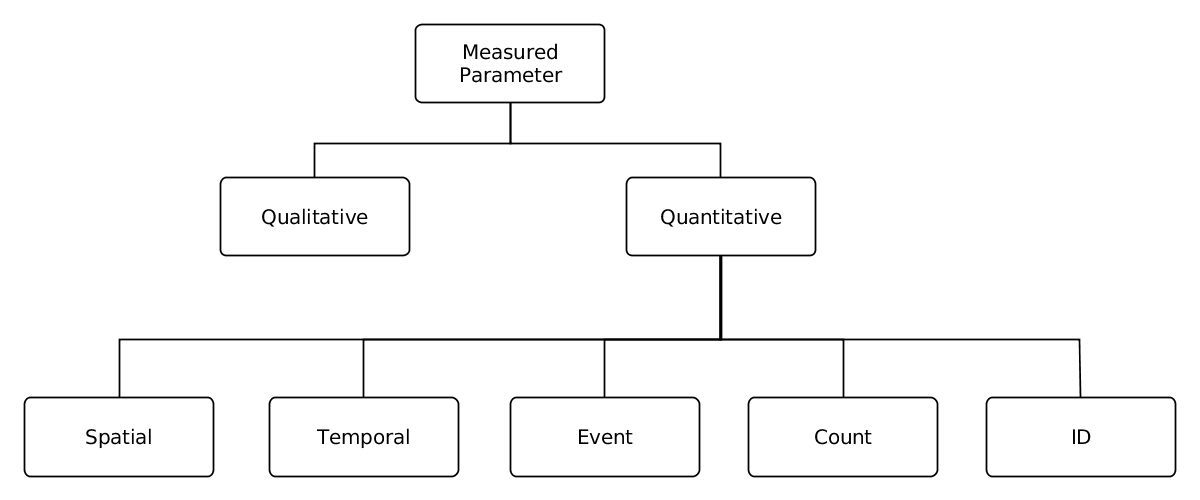
\includegraphics[width=\linewidth]{sensor_platform_param_hierarchy}
\caption{Measured parameter hierarchy \label{fig:sensor_platform_param_hierarchy}}
\end{figure}

There are multiple types of sensors ranging from humans (manual observations entered into a database) to wearable devices (electronic observations automatically streamed to a database). In some cases, multiple types of sensors can collect the same type of information, e.g. a human could manually annotate player paths, albeit tedious compared to computer vision approaches that automatically track players. The model is refined to categorise different types of sensors according to the hierarchy in \figref{fig:sensor_platform_sensor_hierarchy}.

Classes of measured parameters were identified to distinguish between
fundamentally different kinds of unit systems encountered in datasets.
In physics, the theory of relativity shows that space and time
dimensions are intricately related, and hence space and time share
common units (e.g. ``light-years'' describes spatial measurements in
terms of time). However, for the purposes of sport, they can be considered independent. These classes of measured parameters in sport are presented as a hierarchy in \figref{fig:sensor_platform_param_hierarchy}.
Note that each of these types can be either sparse or dense.


Each of these classes are listed in Table \ref{tab:irregular}, along with
required meta-data to describe these measurements. Accuracy is a
critical consideration in description of any measurement. Measurements
on a nominal scale, such as Events and Qualitative measurements, require
specification of the granularity of the scale, in addition to accuracy.

%\clearpage

Dense parameters require additional meta-data to describe the
regularity of the sampling, as listed in Table \ref{tab:regular}. Sequences identifiers are always modelled as dense.
The accuracy, error, and reliability attributes listed in Table \ref{tab:irregular} are optional for dense parameters in cases where
the dense parameter is taken as a definitive (e.g. cell size), and error estimates of measured sparse parameters (e.g. count of players in cell) account for any inaccuracies in observation of the dense parameter (e.g. inaccurate player counts due to ambiguities of the cell boundary).

\begin{table}[h]
\caption{Attributes of Measurements}
\label{tab:irregular}
\begin{tabular}{lll}
\toprule
Measured Param. & Attribute & Example\tabularnewline
\midrule
Spatial & Error Radius & 5 m error radius\tabularnewline
Temporal & Accuracy & $\pm$ 5 sec\tabularnewline
Event & Accuracy & 95\% correct classification\tabularnewline
& Granularity & \{Pass, Tackle, Score\}\tabularnewline
Qualitative & Inter-rate Reliability & Cohen's kappa =
0.9\tabularnewline
& Granularity & \{Easy Pass, Hard Pass\}\tabularnewline
Count & Accuracy & $\pm$ 1\tabularnewline
ID & Accuracy & 98\% correct ID classification\tabularnewline
\bottomrule
\end{tabular}
\end{table}

\begin{table}[h]
\caption{Attributes of Dense Measurements}
\label{tab:regular}
\begin{tabular}{lll}
\toprule
Measured Param. & Attribute & Example\tabularnewline
\midrule
Spatial* & Cell Size & 10 m $\times$ 10 m square cells\tabularnewline
Temporal* & Sample Rate & 10 Hz\tabularnewline
Count* & Bin Size & \{(0,10),(10,20),(20,30),\ldots{}\}\tabularnewline
ID* (Sequence) & Accuracy & 95\% follow correct sequenced\tabularnewline
\bottomrule
\end{tabular}
\end{table}

%\newpage

\subsection{Definitions}\label{definitions}

Using the proposed model, one can now precisely define the difference between various levels of spatio-temporal data. The model can be used to describe either raw data, or processed data ready for visualisation. However, note that transformations during the processing of data
(e.g.~summarisation to reduce data, or calculation of new derived variables) can change the data type.

\begin{itemize}
\item
  \textbf{Event-Count data}: Sensor data dense in Event parameter, and
  sparse/dense in Count parameter.
\item
  \textbf{Spatio-Temporal data}: Sensor platform with a sensor that
  collects any form of Spatial parameter and a sensor that collects any
  form of Temporal parameter. (e.g.~time and distance of a sprint)
\item
  \textbf{Time Dense Spatio-Temporal data}: Sensor data containing
  sparse/dense Spatial parameter, and dense time parameter (e.g.~GPS
  trace).
\item
  \textbf{Space Dense Spatio-Temporal data}: Sensor data containing
  dense Spatial parameter, and sparse/dense time parameter (e.g.~static
  heat-map of time spent in each position).
\item
  \textbf{Space-Time Dense Spatio-Temporal data}: Sensor data containing
  dense Spatial parameter, and dense time parameter (e.g.~heat-map of
  recent events as function of time).
\end{itemize}

% Examples moved to appendix

The model is applied to describe various sport datasets in \appendixref{appendix:modelling}. In particular, the model was used to describe the dataset collected by wearable tracking devices used in this thesis (\appendixsecref{data-collection}). In applying the model, it became apparent that some relevant accuracy details were undocumented in product details, e.g. specifications describing the position accuracy and sample rate, but not how precise the internal clock was\footnote{In the case of GPS devices, satellites broadcast GPS timing information, which allows a theoretical accuracy of 40 nanoseconds. US Government, ``GPS Accuracy,'' 2017. \url{https://www.gps.gov/systems/gps/performance/accuracy/} Accessed:~2019-02-20. However when reporting this information accuracy can be degraded by conversion issues such as improperly accounting for leap seconds.}. An awareness of timing drifts is vital for analysis, as the distance players can move in a second is greater than typical positioning related error. This demonstrates the value of the model in drawing attention to all relevant parameters that could potentially affect the results of the analysis.

\subsection{Conclusion}\label{conclusion-dataclass}

Sport performance datasets contain various forms of spatio-temporal
data. An abstract data model was introduced and associated syntax for describing
the different forms of spatio-temporal data contained in these data
sets. It was demonstrated that the proposed model can be used to describe both
traditional and contemporary sport performance datasets. The model also
revealed missing error estimates that are needed in order to
systematically reason about the data quality. % Future work is needed to
%study meaningful transformations between different datasets.

% \subsection{References}\label{references}
